% !TeX program = pdflatex
% !TeX encoding = UTF-8
% =============================================================================
%  PLANTILLA — Artículo Académico sin Portada
%  Maestría en Urbanismo, UNAM – FES Acatlán
%  Versión 1.0 — Abril 2026
%
%  USO:
%    1. Edita el bloque "PERSONALIZACIÓN" con los datos del entregable.
%    2. Cada palabra clave va dentro de \uline{} separadas por comas.
%    3. Completa las secciones en /secciones/ con tu contenido.
%    4. Agrega tus referencias en referencias.bib.
%    5. Compila con: pdflatex → bibtex → pdflatex → pdflatex
% =============================================================================

\documentclass[12pt,a4paper]{article}

% ═════════════════════════════════════════════════════════════════════════════
%  PERSONALIZACIÓN — Edita solo esta sección para cada nuevo entregable
% ═════════════════════════════════════════════════════════════════════════════
\newcommand{\TituloArticulo}{El aula como entorno inmersivo: experiencia sensorial y cognitiva del autismo}
\newcommand{\Autor}{Hernán Galileo Cabrera Garibaldi}
\newcommand{\Materia}{Didáctica}
\newcommand{\MateriaCorta}{Didáctica — Semestre 2027-1}   % Aparece en el pie
\newcommand{\FechaEntrega}{Noviembre 2026}

% Palabras clave: encierra cada término en \uline{} separado por comas
\newcommand{\PalabrasClave}{%
  \uline{neurodiversidad},\ %
  \uline{autismo},\ %
  \uline{sobrecarga sensorial},\ %
  \uline{enmascaramiento},\ %
  \uline{diseño inclusivo}%
}
% ═════════════════════════════════════════════════════════════════════════════

% =============================================================================
%  1. IDIOMA Y CODIFICACIÓN
% =============================================================================
\usepackage[utf8]{inputenc}
\usepackage[T1]{fontenc}
\usepackage[spanish,es-tabla,es-nodecimaldot]{babel}
\usepackage{csquotes}

% =============================================================================
%  2. LAYOUT BASE
% =============================================================================
\usepackage{geometry}
\geometry{top=2.5cm, bottom=2.5cm, left=3.0cm, right=2.5cm}

% =============================================================================
%  3. PAQUETES ESENCIALES
% =============================================================================
\usepackage{graphicx}
\usepackage{amsmath}
\usepackage{natbib}

% =============================================================================
%  4. PAQUETES ADICIONALES, COLORES Y COMANDOS PERSONALIZADOS
%     Ajusta paleta de colores y comandos en Latex/Comands.tex
% =============================================================================
% =============================================================================
%  Comands.tex — Paquetes adicionales y comandos personalizados
%  Plantilla: Artículo Académico sin Portada
%
%  NOTA: Cargado desde main.tex con % =============================================================================
%  Comands.tex — Paquetes adicionales y comandos personalizados
%  Plantilla: Artículo Académico sin Portada
%
%  NOTA: Cargado desde main.tex con % =============================================================================
%  Comands.tex — Paquetes adicionales y comandos personalizados
%  Plantilla: Artículo Académico sin Portada
%
%  NOTA: Cargado desde main.tex con \input{Latex/Comands}
%        Debe cargarse ANTES de \usepackage{hyperref}
% =============================================================================


% ═════════════════════════════════════════════════════════════════════════════
%  PALETA DE COLORES
%  El tema se carga desde Latex/color-config.tex → Latex/Colores/<tema>.tex
%  Temas disponibles: Institucional | Teal | VerdeOlivo | Purpura | Rojo
%
%  Cambiar el color de este documento:
%    • Permanente: edita \providecommand en Latex/color-config.tex
%    • Una compilación: make Document DIR=<ruta> COLOR=Teal
% ═════════════════════════════════════════════════════════════════════════════
\usepackage[table]{xcolor}
\input{Latex/color-config}            % define \ColorTema (default: Institucional)
\input{Latex/Colores/\ColorTema}      % carga ColorPrincipal y ColorAcento
\definecolor{ColorFondoTabla}{RGB}{240, 240, 240}  % Gris claro para tablas
\definecolor{ColorAlerta}   {RGB}{183,  28,  28}  % Rojo para notas de revisión
% ═════════════════════════════════════════════════════════════════════════════


% =============================================================================
%  1. SUBRAYADO (necesario para palabras clave)
% =============================================================================
\usepackage[normalem]{ulem}   % \uline{} — normalem preserva \emph en cursiva


% =============================================================================
%  2. TABLAS
% =============================================================================
\usepackage{longtable}
\usepackage{array}
\usepackage{booktabs}
\usepackage{tabularx}
\usepackage{multirow}


% =============================================================================
%  3. FIGURAS
%  caption DEBE cargarse antes de hyperref
% =============================================================================
\usepackage{graphicx}
% Ruta de búsqueda de imágenes:
%   img/          → carpeta local del artículo
%   ../../../Img/ → carpeta compartida en raíz del proyecto (escudos UNAM/FES)
\graphicspath{{img/}{../../../Img/}}
\usepackage{caption}
\usepackage{subcaption}
\usepackage{float}
\usepackage{wrapfig}


% =============================================================================
%  4. TIPOGRAFÍA Y ESPACIADO
% =============================================================================
\usepackage{setspace}
\usepackage{enumitem}
\usepackage{microtype}
\usepackage[parfill]{parskip}

% Títulos de sección con color
\usepackage{titlesec}
\titleformat{\section}
  {\large\bfseries\color{ColorPrincipal}}{\thesection.}{0.5em}{}
\titleformat{\subsection}
  {\normalsize\bfseries\color{ColorPrincipal!80!black}}{\thesubsection}{0.5em}{}
\titleformat{\subsubsection}
  {\normalsize\itshape\color{ColorPrincipal!60!black}}{\thesubsubsection}{0.5em}{}


% =============================================================================
%  5. ENCABEZADOS Y PIES DE PÁGINA
% =============================================================================
\usepackage{fancyhdr}
\setlength{\headheight}{25pt}
\addtolength{\topmargin}{-10pt}

% Estilo normal (todas las páginas)
\pagestyle{fancy}
\fancyhf{}
\fancyhead[L]{\footnotesize\color{ColorPrincipal}\textbf{\Materia}}
\fancyhead[R]{\footnotesize\Autor}
\renewcommand{\headrulewidth}{0.6pt}
\renewcommand{\headrule}{{\color{ColorPrincipal}\rule{\linewidth}{0.6pt}}}

% Pie de página: materia y fecha a la izquierda, número a la derecha
\fancyfoot[L]{\footnotesize\color{ColorPrincipal}\MateriaCorta\ —\ \FechaEntrega}
\fancyfoot[R]{\footnotesize\thepage}
\renewcommand{\footrulewidth}{0pt}

% Estilo primera página (mismo encabezado, mismo pie)
\fancypagestyle{primerapagina}{%
  \fancyhf{}
  \fancyhead[L]{\footnotesize\color{ColorPrincipal}\textbf{\Materia}}
  \fancyhead[R]{\footnotesize\Autor}
  \renewcommand{\headrulewidth}{0.6pt}
  \renewcommand{\headrule}{{\color{ColorPrincipal}\rule{\linewidth}{0.6pt}}}
  \fancyfoot[L]{\footnotesize\color{ColorPrincipal}\MateriaCorta\ —\ \FechaEntrega}
  \fancyfoot[R]{\footnotesize\thepage}
  \renewcommand{\footrulewidth}{0pt}
}


% =============================================================================
%  6. BLOQUE DE TÍTULO SIN PORTADA
%     Comando que reemplaza la portada: título + línea + palabras clave.
%     Llamar con \cabeceroarticulo al inicio del documento.
% =============================================================================
\newcommand{\cabeceroarticulo}{%
  \thispagestyle{primerapagina}%
  \vspace*{0.4cm}%
  \noindent{\Large\bfseries \TituloArticulo}\\[0.15cm]%
  {\color{ColorPrincipal}\rule{\textwidth}{2pt}}\\[0.3cm]%
  \noindent\textbf{Palabras Clave:}\ \PalabrasClave%
  \vspace{0.7cm}\par%
}


% =============================================================================
%  7. CONFIGURACIÓN DE FIGURAS
% =============================================================================
\renewcommand*{\thesubfigure}{(\alph{subfigure})}

\captionsetup{
  font            = small,
  labelfont       = bf,
  labelsep        = period,
  justification   = raggedright,
  singlelinecheck = false
}


% =============================================================================
%  8. COMANDOS DE PRESENTACIÓN
% =============================================================================

% Fuente debajo de figura
% Uso: \fuentefigura{Elaboración propia con base en \citep{autor2024}.}
\newcommand{\fuentefigura}[1]{%
  \par\vspace{2pt}{\small\textit{Fuente: #1}}%
}

% Nota al margen de revisión (comentar antes de entrega)
% Uso: \pendiente{Completar con datos de campo}
\newcommand{\pendiente}[1]{%
  \marginpar{\footnotesize\color{ColorAlerta}\textbf{[Pendiente:} #1\textbf{]}}%
}

% Término definido por primera vez
\newcommand{\termino}[1]{\textit{#1}}

% Bloque de cita destacada
% Uso: \citaclave{Texto de la definición clave.}
\newcommand{\citaclave}[1]{%
  \begin{quote}
    \color{ColorPrincipal}\itshape #1
  \end{quote}%
}


% =============================================================================
%  9. ABREVIATURAS — agrega las tuyas aquí
% =============================================================================
\newcommand{\cdmx}{Ciudad de México}
\newcommand{\zmvm}{Zona Metropolitana del Valle de México}
\newcommand{\unam}{Universidad Nacional Autónoma de México}
\newcommand{\gis}{\textsc{gis}}

%        Debe cargarse ANTES de \usepackage{hyperref}
% =============================================================================


% ═════════════════════════════════════════════════════════════════════════════
%  PALETA DE COLORES
%  El tema se carga desde Latex/color-config.tex → Latex/Colores/<tema>.tex
%  Temas disponibles: Institucional | Teal | VerdeOlivo | Purpura | Rojo
%
%  Cambiar el color de este documento:
%    • Permanente: edita \providecommand en Latex/color-config.tex
%    • Una compilación: make Document DIR=<ruta> COLOR=Teal
% ═════════════════════════════════════════════════════════════════════════════
\usepackage[table]{xcolor}
% color-config.tex — Temas: Institucional | Teal | VerdeOlivo | Purpura | Rojo
\providecommand{\ColorTema}{Teal}
            % define \ColorTema (default: Institucional)
\input{Latex/Colores/\ColorTema}      % carga ColorPrincipal y ColorAcento
\definecolor{ColorFondoTabla}{RGB}{240, 240, 240}  % Gris claro para tablas
\definecolor{ColorAlerta}   {RGB}{183,  28,  28}  % Rojo para notas de revisión
% ═════════════════════════════════════════════════════════════════════════════


% =============================================================================
%  1. SUBRAYADO (necesario para palabras clave)
% =============================================================================
\usepackage[normalem]{ulem}   % \uline{} — normalem preserva \emph en cursiva


% =============================================================================
%  2. TABLAS
% =============================================================================
\usepackage{longtable}
\usepackage{array}
\usepackage{booktabs}
\usepackage{tabularx}
\usepackage{multirow}


% =============================================================================
%  3. FIGURAS
%  caption DEBE cargarse antes de hyperref
% =============================================================================
\usepackage{graphicx}
% Ruta de búsqueda de imágenes:
%   img/          → carpeta local del artículo
%   ../../../Img/ → carpeta compartida en raíz del proyecto (escudos UNAM/FES)
\graphicspath{{img/}{../../../Img/}}
\usepackage{caption}
\usepackage{subcaption}
\usepackage{float}
\usepackage{wrapfig}


% =============================================================================
%  4. TIPOGRAFÍA Y ESPACIADO
% =============================================================================
\usepackage{setspace}
\usepackage{enumitem}
\usepackage{microtype}
\usepackage[parfill]{parskip}

% Títulos de sección con color
\usepackage{titlesec}
\titleformat{\section}
  {\large\bfseries\color{ColorPrincipal}}{\thesection.}{0.5em}{}
\titleformat{\subsection}
  {\normalsize\bfseries\color{ColorPrincipal!80!black}}{\thesubsection}{0.5em}{}
\titleformat{\subsubsection}
  {\normalsize\itshape\color{ColorPrincipal!60!black}}{\thesubsubsection}{0.5em}{}


% =============================================================================
%  5. ENCABEZADOS Y PIES DE PÁGINA
% =============================================================================
\usepackage{fancyhdr}
\setlength{\headheight}{25pt}
\addtolength{\topmargin}{-10pt}

% Estilo normal (todas las páginas)
\pagestyle{fancy}
\fancyhf{}
\fancyhead[L]{\footnotesize\color{ColorPrincipal}\textbf{\Materia}}
\fancyhead[R]{\footnotesize\Autor}
\renewcommand{\headrulewidth}{0.6pt}
\renewcommand{\headrule}{{\color{ColorPrincipal}\rule{\linewidth}{0.6pt}}}

% Pie de página: materia y fecha a la izquierda, número a la derecha
\fancyfoot[L]{\footnotesize\color{ColorPrincipal}\MateriaCorta\ —\ \FechaEntrega}
\fancyfoot[R]{\footnotesize\thepage}
\renewcommand{\footrulewidth}{0pt}

% Estilo primera página (mismo encabezado, mismo pie)
\fancypagestyle{primerapagina}{%
  \fancyhf{}
  \fancyhead[L]{\footnotesize\color{ColorPrincipal}\textbf{\Materia}}
  \fancyhead[R]{\footnotesize\Autor}
  \renewcommand{\headrulewidth}{0.6pt}
  \renewcommand{\headrule}{{\color{ColorPrincipal}\rule{\linewidth}{0.6pt}}}
  \fancyfoot[L]{\footnotesize\color{ColorPrincipal}\MateriaCorta\ —\ \FechaEntrega}
  \fancyfoot[R]{\footnotesize\thepage}
  \renewcommand{\footrulewidth}{0pt}
}


% =============================================================================
%  6. BLOQUE DE TÍTULO SIN PORTADA
%     Comando que reemplaza la portada: título + línea + palabras clave.
%     Llamar con \cabeceroarticulo al inicio del documento.
% =============================================================================
\newcommand{\cabeceroarticulo}{%
  \thispagestyle{primerapagina}%
  \vspace*{0.4cm}%
  \noindent{\Large\bfseries \TituloArticulo}\\[0.15cm]%
  {\color{ColorPrincipal}\rule{\textwidth}{2pt}}\\[0.3cm]%
  \noindent\textbf{Palabras Clave:}\ \PalabrasClave%
  \vspace{0.7cm}\par%
}


% =============================================================================
%  7. CONFIGURACIÓN DE FIGURAS
% =============================================================================
\renewcommand*{\thesubfigure}{(\alph{subfigure})}

\captionsetup{
  font            = small,
  labelfont       = bf,
  labelsep        = period,
  justification   = raggedright,
  singlelinecheck = false
}


% =============================================================================
%  8. COMANDOS DE PRESENTACIÓN
% =============================================================================

% Fuente debajo de figura
% Uso: \fuentefigura{Elaboración propia con base en \citep{autor2024}.}
\newcommand{\fuentefigura}[1]{%
  \par\vspace{2pt}{\small\textit{Fuente: #1}}%
}

% Nota al margen de revisión (comentar antes de entrega)
% Uso: \pendiente{Completar con datos de campo}
\newcommand{\pendiente}[1]{%
  \marginpar{\footnotesize\color{ColorAlerta}\textbf{[Pendiente:} #1\textbf{]}}%
}

% Término definido por primera vez
\newcommand{\termino}[1]{\textit{#1}}

% Bloque de cita destacada
% Uso: \citaclave{Texto de la definición clave.}
\newcommand{\citaclave}[1]{%
  \begin{quote}
    \color{ColorPrincipal}\itshape #1
  \end{quote}%
}


% =============================================================================
%  9. ABREVIATURAS — agrega las tuyas aquí
% =============================================================================
\newcommand{\cdmx}{Ciudad de México}
\newcommand{\zmvm}{Zona Metropolitana del Valle de México}
\newcommand{\unam}{Universidad Nacional Autónoma de México}
\newcommand{\gis}{\textsc{gis}}

%        Debe cargarse ANTES de \usepackage{hyperref}
% =============================================================================


% ═════════════════════════════════════════════════════════════════════════════
%  PALETA DE COLORES
%  El tema se carga desde Latex/color-config.tex → Latex/Colores/<tema>.tex
%  Temas disponibles: Institucional | Teal | VerdeOlivo | Purpura | Rojo
%
%  Cambiar el color de este documento:
%    • Permanente: edita \providecommand en Latex/color-config.tex
%    • Una compilación: make Document DIR=<ruta> COLOR=Teal
% ═════════════════════════════════════════════════════════════════════════════
\usepackage[table]{xcolor}
% color-config.tex — Temas: Institucional | Teal | VerdeOlivo | Purpura | Rojo
\providecommand{\ColorTema}{Teal}
            % define \ColorTema (default: Institucional)
\input{Latex/Colores/\ColorTema}      % carga ColorPrincipal y ColorAcento
\definecolor{ColorFondoTabla}{RGB}{240, 240, 240}  % Gris claro para tablas
\definecolor{ColorAlerta}   {RGB}{183,  28,  28}  % Rojo para notas de revisión
% ═════════════════════════════════════════════════════════════════════════════


% =============================================================================
%  1. SUBRAYADO (necesario para palabras clave)
% =============================================================================
\usepackage[normalem]{ulem}   % \uline{} — normalem preserva \emph en cursiva


% =============================================================================
%  2. TABLAS
% =============================================================================
\usepackage{longtable}
\usepackage{array}
\usepackage{booktabs}
\usepackage{tabularx}
\usepackage{multirow}


% =============================================================================
%  3. FIGURAS
%  caption DEBE cargarse antes de hyperref
% =============================================================================
\usepackage{graphicx}
% Ruta de búsqueda de imágenes:
%   img/          → carpeta local del artículo
%   ../../../Img/ → carpeta compartida en raíz del proyecto (escudos UNAM/FES)
\graphicspath{{img/}{../../../Img/}}
\usepackage{caption}
\usepackage{subcaption}
\usepackage{float}
\usepackage{wrapfig}


% =============================================================================
%  4. TIPOGRAFÍA Y ESPACIADO
% =============================================================================
\usepackage{setspace}
\usepackage{enumitem}
\usepackage{microtype}
\usepackage[parfill]{parskip}

% Títulos de sección con color
\usepackage{titlesec}
\titleformat{\section}
  {\large\bfseries\color{ColorPrincipal}}{\thesection.}{0.5em}{}
\titleformat{\subsection}
  {\normalsize\bfseries\color{ColorPrincipal!80!black}}{\thesubsection}{0.5em}{}
\titleformat{\subsubsection}
  {\normalsize\itshape\color{ColorPrincipal!60!black}}{\thesubsubsection}{0.5em}{}


% =============================================================================
%  5. ENCABEZADOS Y PIES DE PÁGINA
% =============================================================================
\usepackage{fancyhdr}
\setlength{\headheight}{25pt}
\addtolength{\topmargin}{-10pt}

% Estilo normal (todas las páginas)
\pagestyle{fancy}
\fancyhf{}
\fancyhead[L]{\footnotesize\color{ColorPrincipal}\textbf{\Materia}}
\fancyhead[R]{\footnotesize\Autor}
\renewcommand{\headrulewidth}{0.6pt}
\renewcommand{\headrule}{{\color{ColorPrincipal}\rule{\linewidth}{0.6pt}}}

% Pie de página: materia y fecha a la izquierda, número a la derecha
\fancyfoot[L]{\footnotesize\color{ColorPrincipal}\MateriaCorta\ —\ \FechaEntrega}
\fancyfoot[R]{\footnotesize\thepage}
\renewcommand{\footrulewidth}{0pt}

% Estilo primera página (mismo encabezado, mismo pie)
\fancypagestyle{primerapagina}{%
  \fancyhf{}
  \fancyhead[L]{\footnotesize\color{ColorPrincipal}\textbf{\Materia}}
  \fancyhead[R]{\footnotesize\Autor}
  \renewcommand{\headrulewidth}{0.6pt}
  \renewcommand{\headrule}{{\color{ColorPrincipal}\rule{\linewidth}{0.6pt}}}
  \fancyfoot[L]{\footnotesize\color{ColorPrincipal}\MateriaCorta\ —\ \FechaEntrega}
  \fancyfoot[R]{\footnotesize\thepage}
  \renewcommand{\footrulewidth}{0pt}
}


% =============================================================================
%  6. BLOQUE DE TÍTULO SIN PORTADA
%     Comando que reemplaza la portada: título + línea + palabras clave.
%     Llamar con \cabeceroarticulo al inicio del documento.
% =============================================================================
\newcommand{\cabeceroarticulo}{%
  \thispagestyle{primerapagina}%
  \vspace*{0.4cm}%
  \noindent{\Large\bfseries \TituloArticulo}\\[0.15cm]%
  {\color{ColorPrincipal}\rule{\textwidth}{2pt}}\\[0.3cm]%
  \noindent\textbf{Palabras Clave:}\ \PalabrasClave%
  \vspace{0.7cm}\par%
}


% =============================================================================
%  7. CONFIGURACIÓN DE FIGURAS
% =============================================================================
\renewcommand*{\thesubfigure}{(\alph{subfigure})}

\captionsetup{
  font            = small,
  labelfont       = bf,
  labelsep        = period,
  justification   = raggedright,
  singlelinecheck = false
}


% =============================================================================
%  8. COMANDOS DE PRESENTACIÓN
% =============================================================================

% Fuente debajo de figura
% Uso: \fuentefigura{Elaboración propia con base en \citep{autor2024}.}
\newcommand{\fuentefigura}[1]{%
  \par\vspace{2pt}{\small\textit{Fuente: #1}}%
}

% Nota al margen de revisión (comentar antes de entrega)
% Uso: \pendiente{Completar con datos de campo}
\newcommand{\pendiente}[1]{%
  \marginpar{\footnotesize\color{ColorAlerta}\textbf{[Pendiente:} #1\textbf{]}}%
}

% Término definido por primera vez
\newcommand{\termino}[1]{\textit{#1}}

% Bloque de cita destacada
% Uso: \citaclave{Texto de la definición clave.}
\newcommand{\citaclave}[1]{%
  \begin{quote}
    \color{ColorPrincipal}\itshape #1
  \end{quote}%
}


% =============================================================================
%  9. ABREVIATURAS — agrega las tuyas aquí
% =============================================================================
\newcommand{\cdmx}{Ciudad de México}
\newcommand{\zmvm}{Zona Metropolitana del Valle de México}
\newcommand{\unam}{Universidad Nacional Autónoma de México}
\newcommand{\gis}{\textsc{gis}}


% =============================================================================
%  5. HIPERVÍNCULOS — siempre al final del preámbulo
% =============================================================================
\usepackage[
    colorlinks = true,
    linkcolor  = ColorPrincipal,
    citecolor  = ColorPrincipal,
    urlcolor   = ColorPrincipal,
    unicode    = true,
    breaklinks = true
]{hyperref}
\hypersetup{
    pdftitle   = {\TituloArticulo},
    pdfauthor  = {\Autor},
    pdfsubject = {Artículo — \Materia, Maestría en Urbanismo UNAM},
    pdfcreator = {pdfLaTeX + natbib/bibtex}
}

% =============================================================================
%  DOCUMENTO
% =============================================================================
\begin{document}
\onehalfspacing

% ── Bloque de título (reemplaza la portada) ───────────────────────────────────
\cabeceroarticulo

% ── Secciones ─────────────────────────────────────────────────────────────────
% =============================================================================
%  1-Objetivos.tex — Objetivos de la sesión
% =============================================================================

\section{Objetivos de la sesión}

Al finalizar la sesión, se espera que quienes participen:

\begin{enumerate}
  \item Se aproximen, mediante una experiencia inmersiva breve y controlada dentro del aula, a algunas de las barreras sensoriales y cognitivas que enfrentan las personas autistas, para comprender el autismo desde la vivencia y no solo desde la definición.
  \item Identifiquen y distingan los conceptos de enmascaramiento (\textit{masking}), hiperfoco, burnout, meltdown y shutdown, a partir de las descripciones de las propias personas autistas.
  \item Reconozcan los estímulos del entorno, como el ruido, la iluminación, la carga visual y las reglas sociales implícitas, que pueden limitar el aprendizaje y la participación, tanto en el aula como en el espacio urbano.
  \item Reflexionen críticamente sobre su papel como urbanistas y docentes en el diseño de espacios y dinámicas que reconozcan la neurodiversidad.
\end{enumerate}

% =============================================================================
%  2-Introduccion.tex — Neurodiversidad, la escuela como entorno sensorial
%  y la inclusión como eliminación de estímulos que limitan el aprendizaje
% =============================================================================
%  NOTA: citas en traducción propia; el original en inglés va en comentario
%        (% ORIG:) junto a cada cita, para verificación.
%  EDITAR: Pellicano y den Houting (2022) — falta número de página exacto de
%          cada cita (se consultó la versión HTML/XML de PMC, sin paginación).
% =============================================================================

\section{Introducción}

Comprender la neurodiversidad es una tarea que atañe tanto a quien enseña como a quien diseña el espacio. \citet{pellicano2022} describen el paradigma de la neurodiversidad como aquel que \enquote{rechaza la idea de que la divergencia respecto a la norma sea un defecto que requiera corrección}\footnote{Todas las citas de este documento son traducción propia del original en inglés.}.
% ORIG: rejects the view that divergence from the norm is a flaw requiring correction
Desde esta perspectiva, los autores sostienen que \enquote{cualquier \enquote{discapacidad} no se entiende mejor como resultado de las características únicas de un individuo, sino como resultado de un entorno que no acomoda eficazmente esas características}, y advierten:
% ORIG: any ‘disability’ is not best understood as the result of an individual’s
%       unique characteristics, but rather as a result of an environment that
%       does not effectively accommodate those characteristics

\begin{displayquote}
Los entornos físicos y sociales en los que todos vivimos están, en general, diseñados para satisfacer las necesidades de quienes se ubican dentro del rango típico del neurodesarrollo; esos mismos entornos son con frecuencia subóptimos, e incluso hostiles, para las personas neurodivergentes, y necesitan ajustarse si se quiere que estas personas lleven una buena vida \citep{pellicano2022}.
\end{displayquote}
% ORIG: The physical and social environments within which we all live are
%       generally designed to meet the needs of those who fall within the
%       typical range of neurodevelopment; these same environments are often
%       suboptimal, and even hostile, for neurodivergent people and need to be
%       adjusted if such people are to lead good lives

Esta lectura coloca al entorno construido en el centro de la discusión. Desde la arquitectura, \citet[p.~143]{mostafa2014} lo plantea así: \enquote{La arquitectura, como ciencia, se ocupa de la manipulación del entorno físico para facilitar ciertas funciones y propiciar comportamientos deseados. Este entorno se compone principalmente de elementos sensoriales: texturas, colores, patrones, acústica, etc.}
% ORIG: Architecture, as a science, deals with the manipulation of the physical
%       environment to facilitate certain functions and elicit intended
%       behavior. This environment is comprised primarily of sensory elements-
%       textures, colors, patterns, acoustics etc.

La escuela es uno de los entornos donde este desajuste se vuelve más evidente. \citet{pellicano2022} la describen en estos términos: \enquote{Los entornos escolares tradicionales y convencionales son un ejemplo de este tipo de entorno: suelen ser físicamente grandes, ruidosos y caóticos, exigen transiciones frecuentes dentro de las clases y entre ellas a lo largo de la jornada escolar, e implican una serie de reglas y expectativas sociales implícitas}.
% ORIG: Traditional, mainstream school settings are an example of one such
%       environment: they are often physically large, noisy and chaotic,
%       require frequent transitions within and between classes throughout the
%       school day, and entail a host of implicit social rules and expectations
Añaden que \enquote{los entornos físicos, como las escuelas, diseñados pensando en las necesidades neurotípicas pueden dejar a las personas autistas en un estado de incomodidad y angustia sensorial, y los entornos sociales regidos por reglas neurotípicas suelen ser igualmente inaccesibles}.
% ORIG: Physical environments, like schools, that are designed with neurotypical
%       needs in mind can leave autistic people in sensory discomfort and
%       distress, and social environments governed by neurotypical rules are
%       often similarly inaccessible

\citet[p.~2]{jones2020} ilustran el mismo fenómeno: \enquote{un niño con hipersensibilidad puede funcionar plenamente en casa, pero experimentar \enquote{discapacidad} al ser colocado en un aula concurrida con estímulos sensoriales significativos, como luces brillantes y niños ruidosos}.
% ORIG: a child with hypersensitivity may be able to fully function at home but
%       may experience ‘disability’ when placed in a busy classroom with
%       significant sensory inputs such as bright lights and noisy children
En su estudio, un testimonio docente lo resume así: \enquote{Con frecuencia los entornos del aula están demasiado saturados visualmente, lo que significa que muchos jóvenes no saben a qué prestar atención y se sienten abrumados} \citep[p.~6]{jones2020}.
% ORIG: Often classroom environments are too visually busy which means many
%       youngsters don't know what to attend to and are overwhelmed
El efecto de la carga visual se ha documentado incluso en población infantil en general: \enquote{Los niños se distrajeron más con el entorno visual, pasaron más tiempo fuera de la tarea y mostraron menores avances en el aprendizaje cuando las paredes estaban muy decoradas que cuando se retiraron las decoraciones} \citep[p.~1362]{fisher2014}.
% ORIG: Children were more distracted by the visual environment, spent more time
%       off task, and demonstrated smaller learning gains when the walls were
%       highly decorated than when the decorations were removed
En el plano auditivo, \citet[p.~564]{ashburner2008} concluyen que \enquote{los niños que tienen dificultad para procesar instrucciones verbales en entornos ruidosos y que a menudo se concentran en conductas de búsqueda sensorial parecen tener mayor probabilidad de un bajo rendimiento académico}.
% ORIG: Children who have difficulty processing verbal instructions in noisy
%       environments and who often focus on sensory-seeking behaviors appear
%       more likely to underachieve academically

Si la barrera está en el entorno, la inclusión empieza por identificarla. Al revisar los factores que modulan el impacto sensorial en el aprendizaje, \citet[p.~11]{jones2020} reportan \enquote{la agencia, la previsibilidad, el diseño del aula, los recursos escolares y el conocimiento del personal como elementos clave para minimizar el impacto de las diferencias sensoriales}.
% ORIG: agency, predictability, classroom design, school resources and staff
%       knowledge as key in minimizing the impact of sensory differences
Esta guía parte de esa premisa: antes de pedir a quien aprende que se adapte, hay que reconocer qué estímulos del aula limitan su aprendizaje. Para ello, la sesión convierte el aula en un entorno inmersivo que permite experimentar, de forma breve y controlada, algunas de esas barreras invisibles.

% =============================================================================
%  3-Conceptos.tex — Masking, hiperfoco y la tríada burnout/meltdown/shutdown
% =============================================================================
%  NOTA: citas en traducción propia; original en comentario (% ORIG:).
%  EDITAR: falta número de página exacto en citas tomadas del texto completo
%          de PMC (Hull et al., Raymaker et al., Ashinoff y Abu-Akel) y del
%          manuscrito aceptado de Wood (paginación distinta a la publicada).
%          Phung et al. y Hours et al. son artículos con número de artículo,
%          sin paginación.
% =============================================================================

\section{Desarrollo teórico: conceptos clave}

Los conceptos de esta sección se presentan, en la medida de lo posible, desde las descripciones de las propias personas autistas recogidas en la investigación, y no desde un listado de síntomas.

\subsection{Masking (enmascaramiento)}

\citet[p.~2519]{hull2017} señalan que \enquote{se plantea como hipótesis que el camuflaje de las características autistas en situaciones sociales es una estrategia común de afrontamiento social en personas adultas con condiciones del espectro autista}, y que \enquote{el camuflaje está motivado por el deseo de encajar con los demás y de establecer vínculos}.
% ORIG: Camouflaging of autistic characteristics in social situations is
%       hypothesised as a common social coping strategy for adults with autism
%       spectrum conditions (ASC).
% ORIG: Camouflaging is motivated by the desire to fit in with others and to
%       make connections.
Entre las técnicas reportadas, una es central para esta sesión: \enquote{forzar y mantener un contacto visual apropiado, o intentar mirar lo más cerca posible de los ojos del otro, fue una técnica compensatoria comúnmente reportada} \citep{hull2017}.
% ORIG: Forcing and maintaining appropriate eye contact, or attempting to look as
%       close to another's eyes as possible, was a common compensatory technique
%       reported.

El costo es alto: \enquote{con mucho, la consecuencia más constante del camuflaje descrita por los participantes fue el agotamiento. El camuflaje fue descrito con frecuencia como algo mental, física y emocionalmente agotador, que requiere una concentración intensa, autocontrol y manejo de la incomodidad} \citep{hull2017}. Un testimonio lo expresa así: \enquote{es mentalmente agotador tener que ser constantemente otra cosa, literalmente no poder ser nunca yo mismo} \citep{hull2017}.
% ORIG: By far the most consistent consequence of camouflaging described by
%       respondents was exhaustion. Camouflaging was frequently described as
%       being mentally, physically, and emotionally draining; requiring
%       intensive concentration, self-control, and management of discomfort.
% ORIG: It's mentally exhausting constantly having to be something else,
%       literally never being able to be myself

\subsection{Hiperfoco}

\citet{ashinoff2021} proponen una definición operativa con cuatro rasgos: \enquote{(1) el hiperfoco es inducido por la implicación en una tarea; (2) el hiperfoco se caracteriza por un estado intenso de atención sostenida o selectiva; (3) durante un estado de hiperfoco hay una percepción disminuida de los estímulos no relevantes para la tarea, y (4) durante un estado de hiperfoco, el desempeño en la tarea mejora}.
% ORIG: (1) hyperfocus is induced by task engagement; (2) hyperfocus is
%       characterized by an intense state of sustained or selective attention;
%       (3) During a hyperfocus state, there is a diminished perception of
%       non-task relevant stimuli; and (4) During a hyperfocus state, task
%       performance improves.

En el contexto escolar, \citet[p.~34]{wood2021} lo aborda desde los intereses intensos: \enquote{tener intereses intensos o \enquote{especiales}, y una tendencia a concentrarse en profundidad con exclusión de otros estímulos, se asocia con la cognición autista, a veces enmarcada como \enquote{monotropismo}. A pesar de algunos inconvenientes y de asociaciones negativas con la repetición no deseada, esta disposición se vincula con una serie de beneficios educativos y de largo plazo para los niños autistas}. De ahí, concluye la autora, \enquote{la importancia de percibir esta disposición como una fortaleza, en lugar de un déficit que deba remediarse de algún modo} \citep{wood2021}.
% ORIG: Having intense or "special" interests and a tendency to focus in depth
%       to the exclusion of other inputs, is associated with autistic
%       cognition, sometimes framed as "monotropism". Despite some drawbacks and
%       negative associations with unwanted repetition, this disposition is
%       linked to a range of educational and longer-term benefits for autistic
%       children.
% ORIG: the importance of perceiving this disposition as a strength
%       (Winter-Messiers 2007) rather than a deficit which must somehow be
%       remedied

El hiperfoco también se describe en el TDAH, condición que con frecuencia acompaña al autismo. \citet{hours2022} indican que, \enquote{según la literatura científica, entre el 50 y el 70\,\% de las personas con trastorno del espectro autista (TEA) presentan también trastorno por déficit de atención e hiperactividad (TDAH) comórbido}, pero aclaran que la nosografía actual \enquote{deja claro que se trata de entidades diferentes, que afectan a los niños y a sus historias de desarrollo de maneras claramente distintas}. Por eso suelen estudiarse a la par, aunque no significan lo mismo. Sobre el TDAH, \citet{ashinoff2021} señalan que, \enquote{aunque el hiperfoco parece contradecir la asociación del TDAH con la inatención y la impulsividad, a menudo se reporta como un estado positivo en personas con TDAH, porque de hecho se implican en tareas durante periodos más largos de lo habitual}.
% ORIG: According to the scientific literature, 50 to 70% of individuals with
%       autism spectrum disorder (ASD) also present with comorbid attention
%       deficit hyperactivity disorder (ADHD).
% ORIG: [The semiology of ASD and ADHD presented in current nosography ...]
%       makes it clear that they are different entities, affecting children
%       and their developmental histories in ways that are clearly distinct.
% ORIG: although hyperfocus is seemingly antithetical to the association of ADHD
%       with inattention and impulsivity, it is often reported as a positive
%       state in individuals with ADHD because they actually engage in tasks
%       for longer periods of time than is typical

\subsection{La tríada del estrés y la regulación}

\citet{phung2021} agrupan cuatro experiencias: \enquote{el burnout, la inercia, el meltdown y el shutdown (BIMS) se han identificado como partes importantes de la vida de algunas personas autistas}. Esta guía retoma tres de ellas.
% ORIG: Burnout, inertia, meltdown, and shutdown (BIMS) have been identified as
%       important parts of some autistic people's lives.

\paragraph{Burnout.} \citet{raymaker2020} lo definen así: \enquote{el burnout autista es un síndrome conceptualizado como resultado del estrés vital crónico y de un desajuste entre expectativas y capacidades sin los apoyos adecuados. Se caracteriza por un agotamiento generalizado y de largo plazo (típicamente de tres meses o más), pérdida de funciones y menor tolerancia a los estímulos}. Entre sus causas, el estudio identifica \enquote{los estresores de la vida (subtemas: enmascaramiento, expectativas, manejo de la discapacidad y cambios vitales) que conducen a una carga acumulada} \citep{raymaker2020}.
% ORIG: Autistic burnout is a syndrome conceptualized as resulting from chronic
%       life stress and a mismatch of expectations and abilities without
%       adequate supports. It is characterized by pervasive, long-term
%       (typically 3+ months) exhaustion, loss of function, and reduced
%       tolerance to stimulus.
% ORIG: life stressors (subthemes: masking, expectations, disability
%       management, and life-changes) that lead to (2) cumulative load

\paragraph{Meltdown.} A partir de investigaciones previas con informantes autistas, \citet{phung2021} lo describen como \enquote{un fenómeno con expresiones variadas en el que los informantes autistas se sienten completamente abrumados, acompañado de una falta de control y de estrés acumulado}, que provoca \enquote{respuestas de ansiedad hacia el exterior y descarga de energía}. Entre sus detonantes mencionan \enquote{demandas sociales, frustración, vergüenza, dificultades de comunicación, detonantes emocionales y estímulos sensoriales aversivos abrumadores}. Una de las personas jóvenes entrevistadas lo describe así: \enquote{eres un pasajero en un viaje de destrucción… y es como ir chocando con un montón de cosas} \citep{phung2021}.
% ORIG: A phenomenon with varying expressions by which autistic informants feel
%       entirely overwhelmed accompanied by a lack of control and cumulative
%       stress
% ORIG: Meltdowns elicit responses of outward anxiety and energy outpour
% ORIG: social demands, frustration, embarrassment, challenges with
%       communication, emotional triggers, and overwhelming aversive sensory
%       stimuli
% ORIG: You're a passenger on a ride of destruction… and it's like hitting a
%       bunch of stuff.

\paragraph{Shutdown.} \enquote{Aunque similares a los meltdowns, los shutdowns se presentan como experiencias más internas, en las que la persona se retira de su entorno y que van acompañadas de dolor emocional} \citep{phung2021}. Su intensidad varía: \enquote{va de leve (p.\,ej., poder caminar y hablar) a severo (p.\,ej., sentirse desconectado de las propias extremidades y adoptar una posición fetal)}. Los autores retoman a Belek, cuya descripción \enquote{enfatiza detonantes como la sobrecarga sensorial y experiencias internas de miedo y parálisis}. En palabras de una persona joven: \enquote{el shutdown es, como, normalmente por estrés: me congelo por completo, no puedo hablar bien, tartamudeo, me congelo literalmente} \citep{phung2021}.
% ORIG: Although similar to meltdowns, shutdowns present as more internal
%       experiences, where the individual withdraws from their surroundings and
%       is accompanied by emotional pain
% ORIG: The degree to which one can function during a shutdown ranges from mild
%       (e.g., being able to walk around and talk) to severe (e.g., feeling
%       detached from your limbs and going into a fetal position)
% ORIG: Belek's description of shutdown emphasizes triggers like sensory
%       overload and internal experiences of fear and paralysis
% ORIG: Shutdown is just, like, usually 'cause of stress, I'll just completely
%       freeze up, I can't really talk, I'll stutter, I'll like literally
%       freeze up.

% =============================================================================
%  4-Actividades.tex — Diseño de la inmersión: cuidados y tres dinámicas
% =============================================================================
%  NOTA: citas en traducción propia; original en comentario (% ORIG:).
%  EDITAR: duración de cada dinámica y materiales específicos (temas de
%          conversación, texto de lectura, audio, iluminación).
% =============================================================================

\section{Actividades didácticas: diseño de la inmersión}

La sesión se organiza en tres dinámicas encadenadas, de modo que cada una aprovecha el estado que deja la anterior: primero la carga social del enmascaramiento, después la explicación conceptual y, al final, la carga sensorial.

\subsection{Consideraciones de cuidado}

Las simulaciones de discapacidad tienen límites documentados. \citet[p.~324]{nario2017} concluyen que \enquote{simular discapacidades promueve el malestar y no mejora las actitudes hacia las personas con discapacidad, lo que socava los esfuerzos por mejorar la integración, aun cuando los participantes reportan mayor preocupación empática y \enquote{comprensión de cómo es la experiencia de la discapacidad}}.
% ORIG: Simulating disabilities promotes distress and fails to improve attitudes
%       toward disabled people, undermining efforts to improve integration even
%       while participants report more empathetic concern and "understanding of
%       what the disability experience is like."
Por ello, esta sesión no pretende reproducir la vivencia autista, sino hacer visible el papel del entorno. La inmersión se acompaña de las voces de personas autistas (sección~3) y cierra con una reflexión sobre el diseño de espacios y metodologías (sección~5). Antes de iniciar:

\begin{itemize}
  \item Se explica la dinámica y se pide el consentimiento del grupo; la participación es voluntaria.
  \item Se avisa con anticipación del uso de luces y sonido intensos, y se pregunta si alguien tiene fotosensibilidad, epilepsia u otra condición que lo desaconseje.
  \item Se considera que en el grupo puede haber personas neurodivergentes, con o sin diagnóstico, para quienes la sobrecarga no es una simulación.
  \item Se permite salir del aula o retirarse de la actividad en cualquier momento, sin necesidad de justificarlo.
\end{itemize}

\subsection{Dinámica 1: El peso de la máscara}

\textbf{Propósito.} Experimentar el costo energético del enmascaramiento descrito en la sección~3.1. La dinámica funciona como metáfora visual y cognitiva: obliga a una persona a sostener una fachada de amabilidad, empatía y normalidad (sonreír bajo la máscara, mantener el contacto visual) mientras procesa información abrumadora e incomprensible con un límite de tiempo estricto. Con ello busca aproximar la sobrecarga de procesamiento y la ansiedad de \enquote{no encajar} en una interacción social normativa.

\textbf{Organización.} El grupo trabaja en parejas. La \textbf{Persona~1} lee el guion proyectado; la \textbf{Persona~2} lleva puesta una máscara blanca física y responde. Cada tema consta de tres intercambios, con una duración aproximada de 2 a 3 minutos. El contraste es deliberado: cada conector suena a charla casual de pasillo, pero desemboca en una pregunta técnica imposible de responder en 10 segundos.
% EDITAR: número de temas por pareja y si los roles se intercambian.

\textbf{Regla de oro para la Persona~1.} Leer el conector de forma muy natural y casual. Inmediatamente después, lanzar la pregunta técnica sin cambiar el tono de voz, como si preguntara la hora.

\textbf{Regla para la Persona~2.} Con la máscara puesta, mantener el contacto visual. Tiene máximo 10 segundos para responder con amabilidad, asintiendo y fingiendo que entiende perfectamente. Si se traba, tartamudea o guarda silencio más de 10 segundos, pierde la dinámica.

\subsubsection*{Guion de conversación}

\begin{enumerate}[label=\textbf{Tema \arabic*.}, wide=0pt, leftmargin=0pt, itemsep=0.6em]

  \item \textbf{Bioquímica celular (el ciclo de Krebs)}
  \begin{enumerate}[label=\alph*), leftmargin=1.8em, itemsep=0.3em]
    \item \textit{Conector:} \enquote{Oye, fíjate que hoy en la mañana me tomé un café y me dio muchísima energía de golpe, lo que me hizo pensar en cómo nuestros cuerpos procesan la energía de los alimentos. Es súper interesante, ¿no?}\par
    \textit{Pregunta:} \enquote{A propósito de eso, ¿me podrías explicar detalladamente cómo la enzima isocitrato deshidrogenasa cataliza la descarboxilación oxidativa en el tercer paso del ciclo de Krebs?}
    \item \textit{Conector:} \enquote{¿Ya comiste? Yo me compré unos tacos de canasta en la entrada; nada como un buen desayuno para aguantar todo el día.}\par
    \textit{Pregunta:} \enquote{Y hablando de aguantar, ¿cuántas moléculas de ATP se obtienen en total por cada molécula de glucosa al sumar la glucólisis, el ciclo de Krebs y la fosforilación oxidativa, y por qué los libros no se ponen de acuerdo en la cifra?}
    \item \textit{Conector:} \enquote{Mi tía está a dieta keto y dice que ya casi no come pan, que ahora su cuerpo \enquote{quema grasa} en lugar de azúcar.}\par
    \textit{Pregunta:} \enquote{¿Y tú cómo explicarías por qué, durante la cetosis, cuando escasea el oxalacetato, el acetil-CoA se desvía hacia la formación de cuerpos cetónicos en lugar de entrar al ciclo de Krebs?}
  \end{enumerate}

  \item \textbf{Física cuántica (la ecuación de Schrödinger)}
  \begin{enumerate}[label=\alph*), leftmargin=1.8em, itemsep=0.3em]
    \item \textit{Conector:} \enquote{Qué loco está el clima hoy, ¿verdad? Siento que es súper impredecible, como que un día hace calor y al otro llueve, casi como el comportamiento de las partículas subatómicas.}\par
    \textit{Pregunta:} \enquote{Me quedé con la duda, ¿cómo describirías exactamente la evolución temporal del estado cuántico de un sistema físico aislado usando la formulación hamiltoniana de la ecuación de Schrödinger?}
    \item \textit{Conector:} \enquote{Mi gato se la pasa metido en cajas, de verdad; ayer se metió en la de unos zapatos y no había forma de sacarlo.}\par
    \textit{Pregunta:} \enquote{Eso me recordó: ¿me explicas cómo el experimento mental del gato de Schrödinger ilustra el problema de la medición, y por qué la decoherencia no termina de resolverlo?}
    \item \textit{Conector:} \enquote{Fíjate que se me fue el internet toda la noche; dicen que en unos años todo va a funcionar con computadoras cuánticas.}\par
    \textit{Pregunta:} \enquote{¿Cómo se representa un qubit en la esfera de Bloch, y qué significa físicamente que su estado sea una superposición de los estados cero y uno?}
  \end{enumerate}

  \item \textbf{Lingüística estructural (el esperanto)}
  \begin{enumerate}[label=\alph*), leftmargin=1.8em, itemsep=0.3em]
    \item \textit{Conector:} \enquote{Ayer estaba viendo una serie en Netflix con subtítulos en otro idioma y pensé en lo difícil que es comunicarnos a veces. Dicen que el esperanto se inventó para solucionar eso y unir al mundo.}\par
    \textit{Pregunta:} \enquote{Por cierto, tú que eres súper empático, ¿me puedes conjugar el verbo \enquote{leer} (\textit{legi}) en tiempo condicional, futuro y participio pasivo en esperanto, y darme un ejemplo rápido en una oración compuesta?}
    \item \textit{Conector:} \enquote{Mi sobrino está aprendiendo inglés con una app y se la pasa diciendo palabras raras a la hora de la comida.}\par
    \textit{Pregunta:} \enquote{¿Y me podrías explicar cómo funciona el acusativo en esperanto, con la terminación \textit{-n}, y por qué permite cambiar el orden de las palabras sin cambiar el significado de la oración?}
    \item \textit{Conector:} \enquote{El otro día alguien me habló en portugués en el metro y medio le entendí; los idiomas parecidos se entienden un poco, ¿no?}\par
    \textit{Pregunta:} \enquote{Ya que estamos, ¿qué diferencia hay entre los sufijos \textit{-et-} y \textit{-eg-} en esperanto, y cómo transformarías \textit{domo} (casa) para decir \enquote{casita} y \enquote{mansión}?}
  \end{enumerate}

  \item \textbf{Ingeniería aeroespacial (mecánica orbital)}
  \begin{enumerate}[label=\alph*), leftmargin=1.8em, itemsep=0.3em]
    \item \textit{Conector:} \enquote{El tráfico para llegar aquí a la UNAM estuvo terrible, a veces desearía poder ir volando o teletransportarme como en las películas de ciencia ficción. A veces me quedo mirando el cielo y los satélites.}\par
    \textit{Pregunta:} \enquote{Justo pensaba en eso: si un satélite está en una órbita elíptica, ¿cuál es el cálculo exacto de la ecuación vis-viva para determinar su velocidad justo en el momento del perigeo?}
    \item \textit{Conector:} \enquote{Este fin vi un video de un cohete de esos que regresan y aterrizan solitos; está impresionante cómo avanza la tecnología.}\par
    \textit{Pregunta:} \enquote{¿Cuál es la ecuación de Tsiolkovski para el cambio de velocidad de un cohete, y cómo influye en ella la relación entre su masa inicial y su masa final?}
    \item \textit{Conector:} \enquote{Anoche se veía la Luna enorme desde la azotea; mi mamá dice que así se ve cuando está más cerca.}\par
    \textit{Pregunta:} \enquote{Por cierto, ¿cómo calcularías el periodo orbital de un satélite a partir de su semieje mayor con la tercera ley de Kepler, y qué le pasa a ese periodo si duplicas la distancia?}
  \end{enumerate}

  \item \textbf{Matemáticas avanzadas (la hipótesis de Riemann)}
  \begin{enumerate}[label=\alph*), leftmargin=1.8em, itemsep=0.3em]
    \item \textit{Conector:} \enquote{Fui al súper a comprar unas cosas y al ver el ticket me puse a pensar en cómo los números y las matemáticas rigen todo nuestro mundo, hasta en las cosas más simples.}\par
    \textit{Pregunta:} \enquote{Hablando de eso, ¿me podrías explicar la relación exacta entre los ceros no triviales de la función zeta de Riemann y la distribución analítica de los números primos?}
    \item \textit{Conector:} \enquote{Estoy pagando el celular a meses sin intereses y la verdad ya ni sé cuánto llevo pagado.}\par
    \textit{Pregunta:} \enquote{Oye, ¿y cómo demostrarías con el argumento de Euclides que hay infinitos números primos, y por qué la serie de los inversos de los primos diverge?}
    \item \textit{Conector:} \enquote{Mi sobrina tiene tarea de fracciones y me pidió ayuda; yo ya no me acuerdo de nada de la secundaria.}\par
    \textit{Pregunta:} \enquote{¿Me puedes explicar por qué la suma $1 + 2 + 3 + 4 + \cdots$ se asocia con $-1/12$ mediante la continuación analítica de la función zeta?}
  \end{enumerate}

  \item \textbf{Neuroanatomía (los nervios craneales)}
  \begin{enumerate}[label=\alph*), leftmargin=1.8em, itemsep=0.3em]
    \item \textit{Conector:} \enquote{Hoy me levanté con un dolor de cabeza horrible, justo por la mandíbula y el ojo. Me tomé una pastilla, pero me puse a leer en el celular sobre cómo están conectados los nervios de la cara.}\par
    \textit{Pregunta:} \enquote{Y ya que estamos platicando de eso, ¿podrías trazarme la ruta anatómica exacta del nervio trigémino, desde su núcleo en el tronco encefálico hasta la inervación de sus tres ramas principales?}
    \item \textit{Conector:} \enquote{Fui al dentista la semana pasada y me pusieron anestesia; estuve con media cara dormida toda la tarde.}\par
    \textit{Pregunta:} \enquote{¿De qué rama del trigémino sale el nervio alveolar inferior que se bloquea con la anestesia dental, y por qué también se adormecen la mitad del labio y la barbilla?}
    \item \textit{Conector:} \enquote{Ayer me dio tanta risa un meme que me dolió la cara de tanto reírme.}\par
    \textit{Pregunta:} \enquote{¿Qué diferencia hay entre el nervio facial y el trigémino en el control de la expresión facial y de la sensibilidad de la cara, y qué número de par craneal es cada uno?}
  \end{enumerate}

  \item \textbf{Teoría musical avanzada (el microtonalismo)}
  \begin{enumerate}[label=\alph*), leftmargin=1.8em, itemsep=0.3em]
    \item \textit{Conector:} \enquote{Venía escuchando una canción súper pegajosa en Spotify y me di cuenta de que casi todas las canciones pop suenan igual. Creo que tiene que ver con que siempre usamos los mismos instrumentos y la misma afinación.}\par
    \textit{Pregunta:} \enquote{Oye, ¿tú sabes cómo se calcularía matemáticamente la diferencia en \textit{cents} entre una coma pitagórica y una coma sintónica dentro de un sistema de afinación justa?}
    \item \textit{Conector:} \enquote{Mi vecino está aprendiendo a tocar la guitarra y se la pasa afinándola cada cinco minutos.}\par
    \textit{Pregunta:} \enquote{¿Y por qué en el temperamento igual de doce notas la quinta no es exactamente la proporción 3/2, y por cuántos \textit{cents} se desvía?}
    \item \textit{Conector:} \enquote{El otro día escuché música árabe en un restaurante y sentí que sonaba \enquote{desafinada}, pero bonita.}\par
    \textit{Pregunta:} \enquote{¿Cómo se usan los cuartos de tono en el sistema de \textit{maqam} árabe, y cuántos \textit{cents} mide un cuarto de tono en un temperamento de 24 notas por octava?}
  \end{enumerate}

\end{enumerate}

\textbf{Vínculo con la teoría.} La dinámica reproduce una de las técnicas compensatorias documentadas por \citet{hull2017}, forzar y mantener el contacto visual, y pone en juego la motivación que los mismos autores identifican detrás del camuflaje: el deseo de encajar con los demás. La máscara hace visible, de forma literal, el esfuerzo que el enmascaramiento oculta, y el cansancio que deja es el punto de partida de la siguiente dinámica.

\subsection{Diseño sonoro de la inmersión}
\label{sec:audio}

El audio que acompaña la Dinámica~3 es una composición propia, editada en Audacity a partir de grabaciones de ambiente, guitarras, sintetizadores y tonos de tinnitus obtenidos de Freesound. Su utilidad es construir la sobrecarga por acumulación: la intensidad no depende solo del volumen, sino de la densidad y del tipo de estímulos que se van sumando, como ocurre en un día escolar en el que las fuentes de ruido se superponen sin pausa.
% EDITAR: verificar licencias de los sonidos de Freesound (CC0 / CC BY) y,
%         si alguna lo requiere, agregar créditos.

\textbf{Formato.} Archivo \texttt{Audio\_Final\_Prueba.wav}, en formato WAV PCM sin compresión, estéreo, a 48\,kHz y 16 bits. Dura 18:58 minutos (1138.6\,s) y pesa cerca de 219\,MB.

\textbf{Configuración.} La mezcla se compone de siete capas que entran de forma escalonada (tabla~\ref{tab:capas}).

\begin{table}[htbp]
\centering
\small
\caption{Capas del audio de la Dinámica~3.}
\label{tab:capas}
\begin{tabularx}{\textwidth}{@{}l X X l@{}}
\toprule
\textbf{Capa} & \textbf{Material} & \textbf{Tratamiento} & \textbf{Presencia} \\
\midrule
Base ambiental & Loop propio de 2:21 min, repetido cinco veces & Ecualización; versión alterna 8.8\,\% más lenta y cerca de 1.5 semitonos más grave & 0:00 -- 11:48 \\
Tinnitus golpeado & Tinnitus con pasos, en intervalos de 16\,s & Distorsión y ganancia alta & 0:14 -- 14:38 \\
Guitarras & Dos grabaciones de retroalimentación (\textit{feedback}) & Compresión en una de ellas & 1:55 -- 12:43 \\
Ambiente ominoso & Ambiente grave y profundo & Filtro pasa altos & 4:52 -- 10:56 \\
Sintetizadores & Drone de bajo con caos agudo y textura \enquote{spooks} & Ecualización & 5:13 -- 13:44 \\
Tinnitus agudo & Tono de 10\,kHz y tinnitus continuo & --- & 10:34 -- 15:59 \\
Calle & Mariachis tocando \textit{La Bamba} con arpa en la Plaza Garibaldi & Reverberación y ecualización & 13:58 -- 18:58 \\
\bottomrule
\end{tabularx}
\end{table}

\textbf{Análisis.} La escalada no es lineal, sino por oleadas. Durante los primeros cinco minutos el nivel medio se mantiene entre $-33$ y $-37$\,dBFS. A partir del minuto 5 alterna minutos más intensos, de cerca de $-23.5$\,dBFS (minutos 6, 8 y 10), con otros de alrededor de $-32$\,dBFS. Entre los minutos 12 y 13 predominan las frecuencias agudas de los tinnitus: un indicador de brillo, la tasa de cruces por cero, llega a triplicar su valor inicial. Del minuto 14 al 18 el audio alcanza su meseta más alta, cerca de $-20$\,dBFS, unos 13\,dB por encima del inicio. No hay muestras recortadas, y el pico máximo es de $-1.6$\,dBFS. Por la presencia de tonos agudos y de niveles altos sostenidos, el volumen se calibra en el aula antes de la sesión (sección~4.1).

\textbf{Final del audio.} A partir del minuto 16 solo queda la grabación de calle. En el último minuto el nivel desciende hasta cerca de $-30$\,dBFS, y el archivo termina en torno a $-37$\,dBFS, sin desvanecerse hasta el silencio. Este cierre traslada la sobrecarga del aula al espacio urbano y conecta la dinámica con el objeto de estudio del urbanismo. El ruido blanco y la pantalla en blanco del corte no forman parte del archivo: se activan al terminar la escalada (sección~\ref{sec:dinamica3}).
% EDITAR: confirmar cómo se reproduce el ruido blanco (archivo aparte o en vivo).

\subsection{Dinámica 2: Entendiendo la teoría a través del cansancio}

\textbf{Propósito.} Presentar los conceptos de la sección~3 mientras el grupo conserva el desgaste mental de la dinámica anterior.

\textbf{Desarrollo.} Se exponen el enmascaramiento, el hiperfoco y la tríada burnout, meltdown y shutdown. El cansancio de la Dinámica 1 sirve como referencia concreta: el grupo puede contrastarlo con la definición de burnout de \citet{raymaker2020}, que habla de un agotamiento \enquote{de largo plazo (típicamente de tres meses o más)}. El contraste entre unos minutos de máscara y meses de carga acumulada da escala a la experiencia.

\subsection{Dinámica 3: Día normal en la escuela (clímax sensorial)}
\label{sec:dinamica3}

\textbf{Propósito.} Hacer perceptible la sobrecarga sensorial descrita en la Introducción, y representar la escalada hacia un meltdown y el retiro propio de un shutdown.

\textbf{Desarrollo.} La dinámica avanza en tres fases sincronizadas con el audio (sección~\ref{sec:audio}). En cada una aumentan a la vez la dificultad del texto y la carga sensorial. La Fase~1 usa un fragmento del Canto IX de la \textit{Odisea}, la llegada de Odiseo y sus hombres a la cueva del cíclope Polifemo: la épica clásica, con su métrica antigua, sus epítetos y su redacción en cantos, resulta densa y poco intuitiva para el lector actual, y funciona como un estímulo complejo que el grupo debe decodificar. La Fase~2 usa el capítulo 34 de \textit{Rayuela}, en el que Cortázar intercala, línea por línea, el texto de una novela tradicional con los pensamientos de Horacio Oliveira. La Fase~3 usa el capítulo 68, escrito en el lenguaje inventado de la novela, el glíglico. Cada fase se proyecta en tres diapositivas.

\subsubsection*{Fase 1: hiperfoco funcionando bien}

Esta fase se proyecta durante los primeros minutos del audio, cuando la base ambiental de oficina y pasillo apenas se percibe. Representa el hiperfoco en un entorno que lo permite: los rasgos (3) y (4) de la definición de \citet{ashinoff2021}, una percepción disminuida de los estímulos no relevantes y un mejor desempeño en la tarea, ayudan a filtrar el adorno del texto y a extraer su contenido. Ilustra lo que \citet{wood2021} plantea al proponer esta disposición como una fortaleza y no como un déficit.
% EDITAR: confirmar intervalo del audio (propuesta: 0:00 – 1:55, antes de que
%         entren las guitarras; solo suenan la base y el tinnitus intermitente).

\textbf{Diapositiva 1: el estímulo denso.} Fondo claro, de pergamino o color neutro, con un bloque largo de texto en versos que puede parecer intimidante a primera vista (figura~\ref{fig:fase1}). Se pide al grupo que lea el texto e intente retener los detalles, mientras el ruido de fondo comienza a sonar suavemente.

\begin{figure}[H]
  \centering
  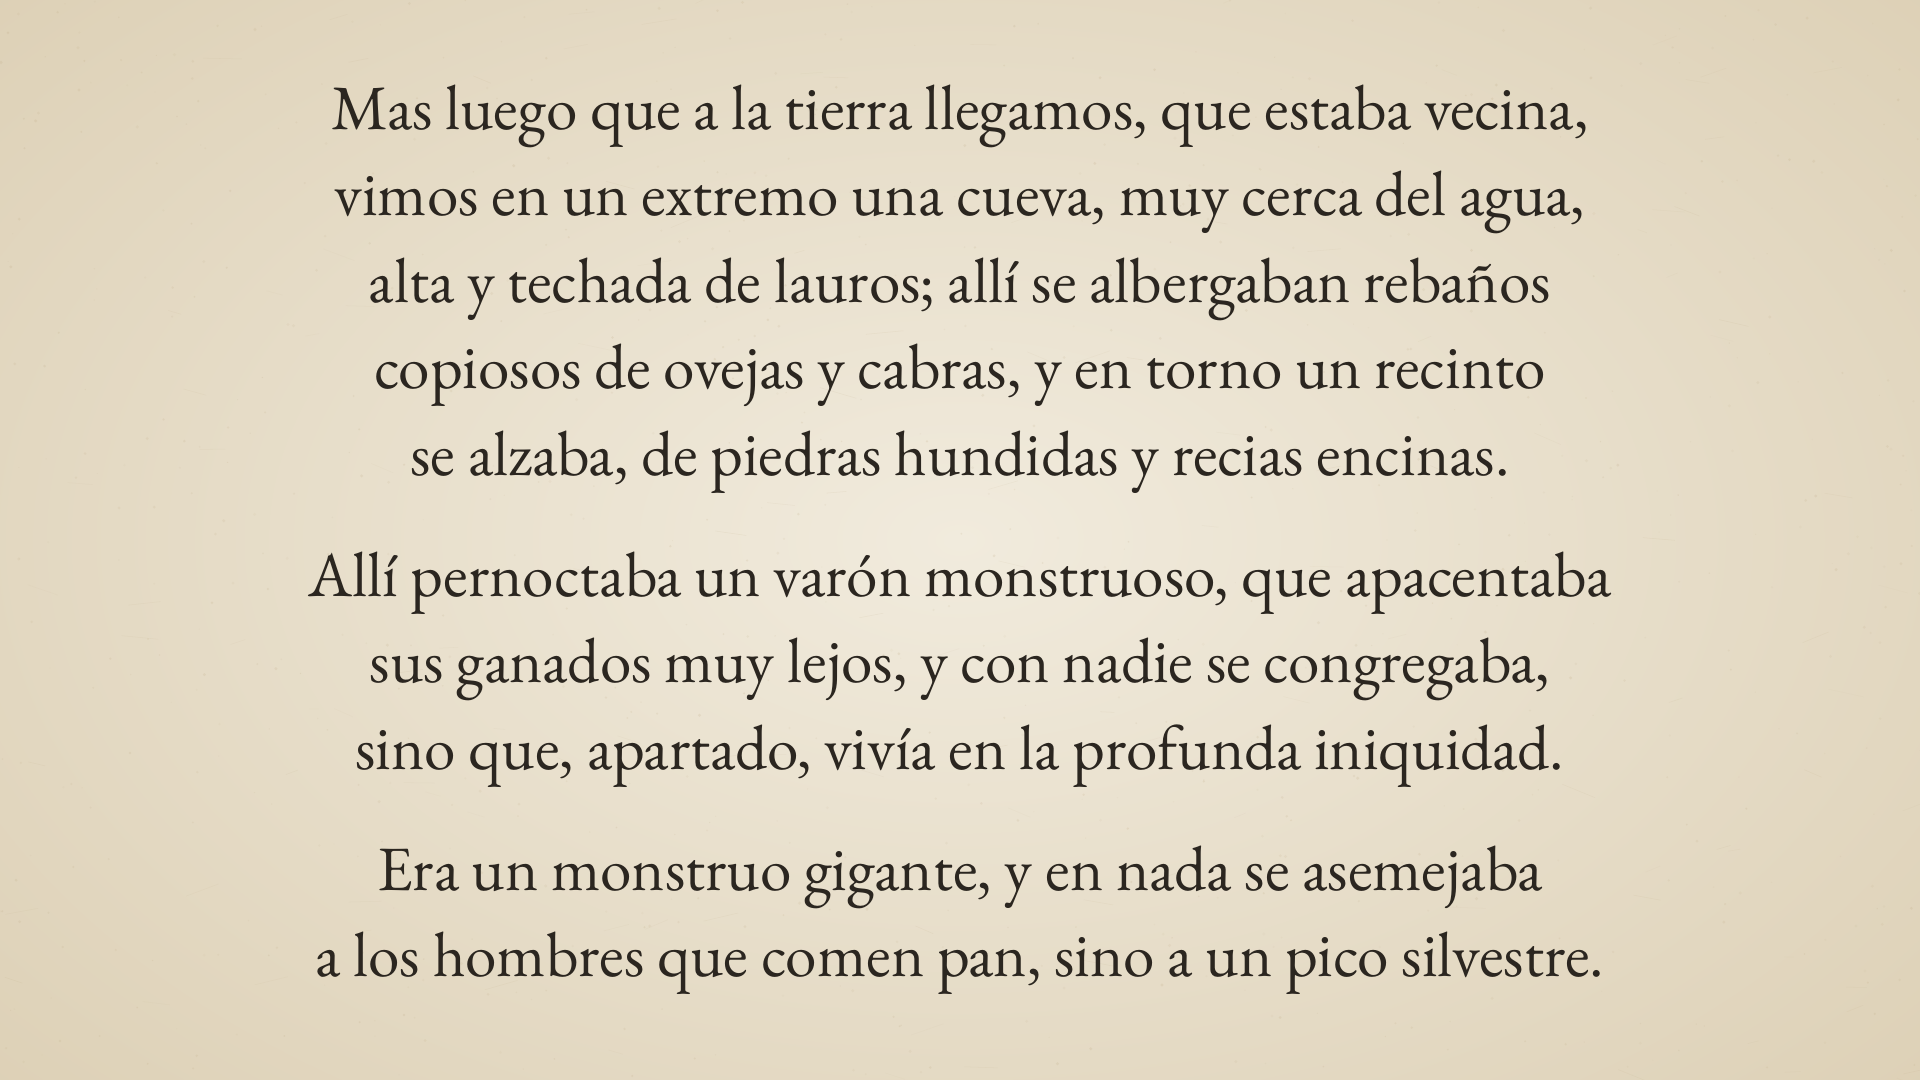
\includegraphics[width=0.85\textwidth]{Resources/img/Dinamica3/Fase1/Dinamica3_Fase1_Diapositiva1.png}
  \caption{Diapositiva 1 de la Fase 1: el estímulo denso.}
  \label{fig:fase1}
  \fuentefigura{Elaboración propia. Texto adaptado del Canto IX de la \textit{Odisea}, vv.~181--192; traducción de referencia: \citet{homero1910}.}
\end{figure}

\textbf{Diapositiva 2: el filtro del hiperfoco.} El fondo cambia bruscamente a un efecto \textit{bokeh}: el texto se oscurece o se desenfoca sutilmente. Ciertas frases clave se iluminan en un color brillante y, junto a ellas, aparecen etiquetas con su traducción directa (figura~\ref{fig:fase1d2}). Se explica que el hiperfoco permite ignorar la \enquote{paja} o el adorno social y literario para ir directo al núcleo de la información, organizando los datos de forma lógica.

\begin{figure}[H]
  \centering
  \includegraphics[width=0.85\textwidth]{Resources/img/Dinamica3/Fase1/Dinamica3_Fase1_Diapositiva2.png}
  \caption{Diapositiva 2 de la Fase 1: el filtro del hiperfoco.}
  \label{fig:fase1d2}
  \fuentefigura{Elaboración propia. Texto adaptado del Canto IX de la \textit{Odisea}, vv.~181--192; traducción de referencia: \citet{homero1910}.}
\end{figure}

\textbf{Diapositiva 3: el resultado procesado.} Fondo completamente oscuro y limpio, con texto grande y centrado en lenguaje cotidiano, sin adornos. Se explica que así se representa la información una vez procesada mediante el hiperfoco: el caos literario quedó ordenado en un sistema claro y útil (figura~\ref{fig:fase1d3}).

\begin{figure}[H]
  \centering
  \includegraphics[width=0.85\textwidth]{Resources/img/Dinamica3/Fase1/Dinamica3_Fase1_Diapositiva3.png}
  \caption{Diapositiva 3 de la Fase 1: el resultado procesado.}
  \label{fig:fase1d3}
  \fuentefigura{Elaboración propia.}
\end{figure}

\subsubsection*{Fase 2: hiperfoco funcionando bien ante un texto más complejo}

Esta fase se proyecta con el audio en su punto medio. Su propósito es mostrar cómo una mente enfocada puede filtrar el \enquote{ruido} y extraer patrones lógicos de un texto complejo. El fragmento corresponde a las primeras 16 líneas del capítulo 34 \citep[p.~212]{cortazar1963}, con los cortes de línea, los guiones y las cursivas de la edición: las líneas impares pertenecen a la novela tradicional y las pares, a los pensamientos de Oliveira.
% EDITAR: confirmar intervalo del audio (propuesta: 4:52 – 10:34, ambiente
%         ominoso, sintetizadores y «spooks»).

\textbf{Diapositiva 1: lectura normal, estímulo confuso.} El texto intercalado se presenta tal cual lo escribió Cortázar, sobre el mismo pergamino de la Fase~1 (figura~\ref{fig:fase2d1}). Se pide al grupo que lo lea de corrido, lo que simula la dificultad inicial de lectura.

\begin{figure}[H]
  \centering
  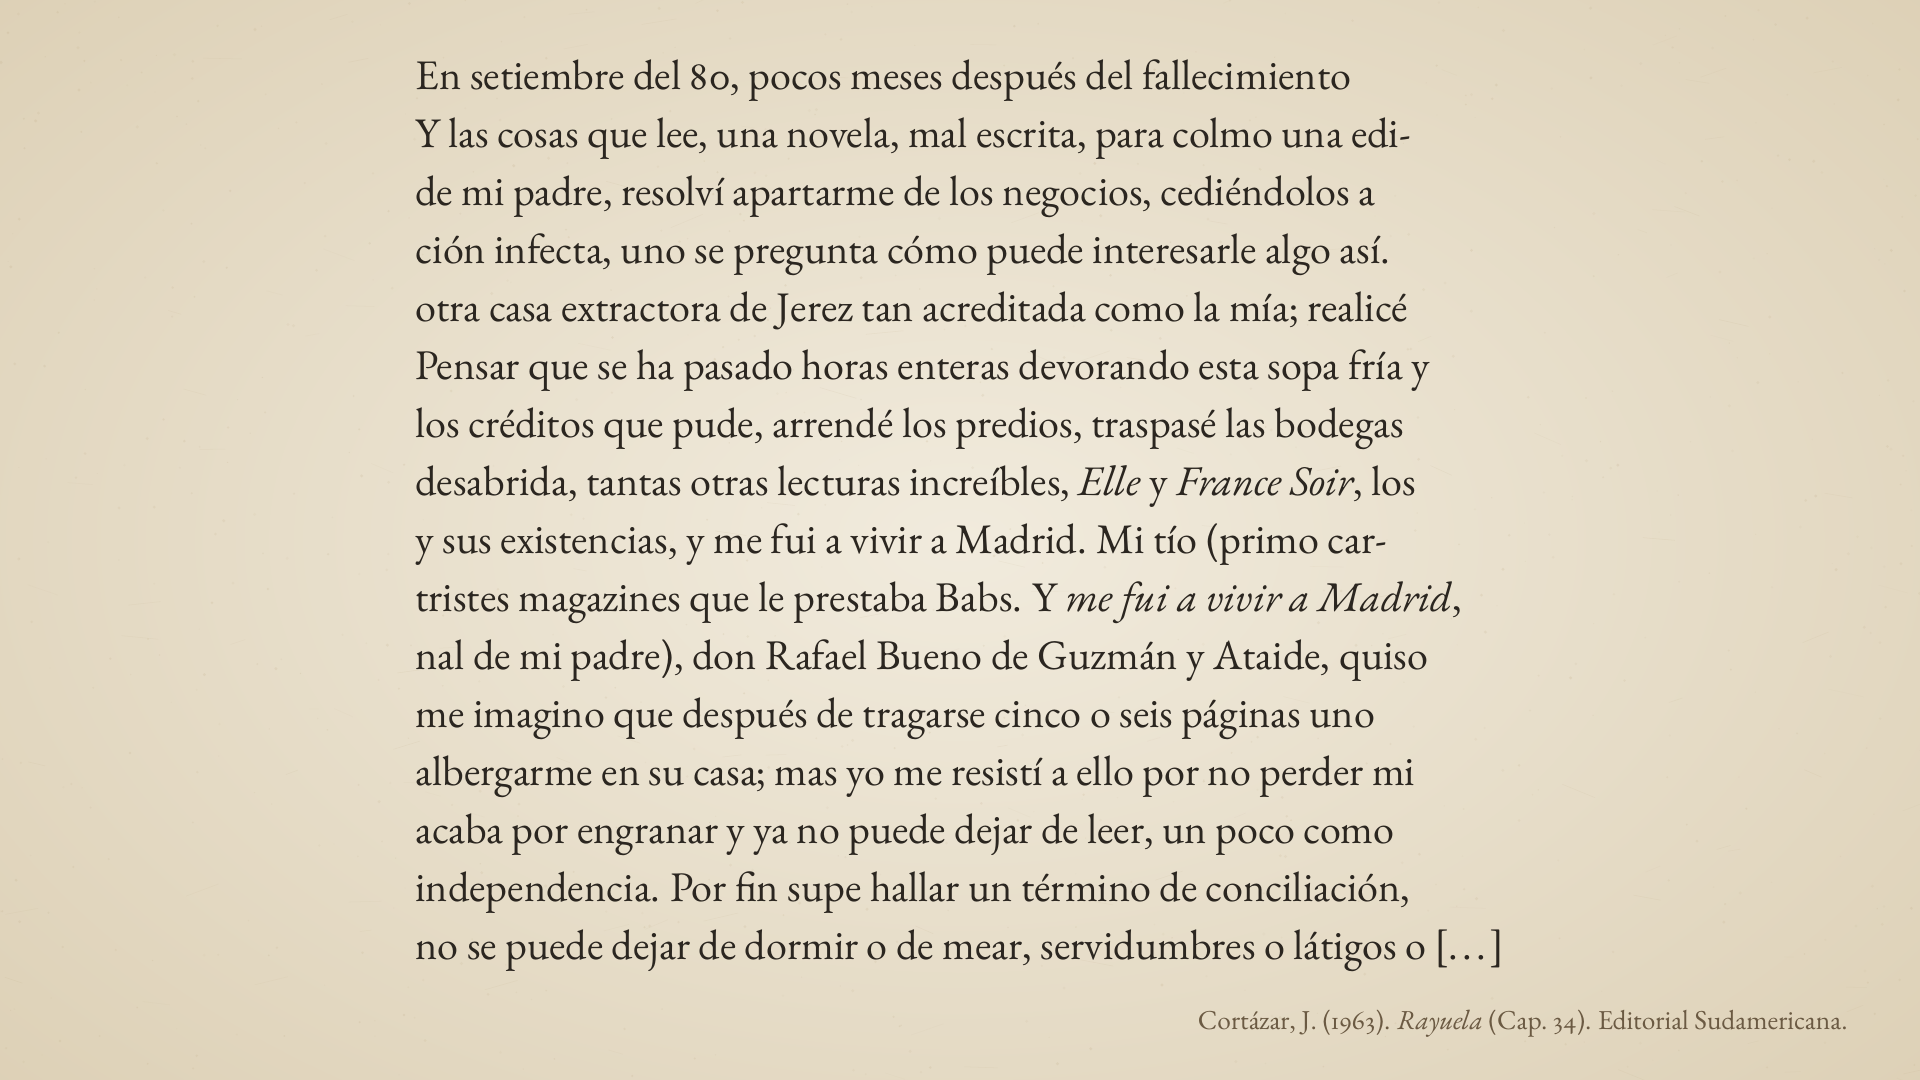
\includegraphics[width=0.85\textwidth]{Resources/img/Dinamica3/Fase2/Dinamica3_Fase2_Diapositiva1.png}
  \caption{Diapositiva 1 de la Fase 2: el texto intercalado del capítulo 34.}
  \label{fig:fase2d1}
  \fuentefigura{Elaboración propia. Texto: \citet[cap.~34, p.~212]{cortazar1963}.}
\end{figure}

\textbf{Diapositiva 2: el filtro del hiperfoco.} Sobre el mismo fondo con bokeh sutil, las líneas de la novela se difuminan en gris, mientras los pensamientos de Oliveira quedan nítidos y resaltados en primer plano (figura~\ref{fig:fase2d2}). Se explica que el filtro separa los dos hilos del texto y deja pasar solo el que interesa.

\begin{figure}[H]
  \centering
  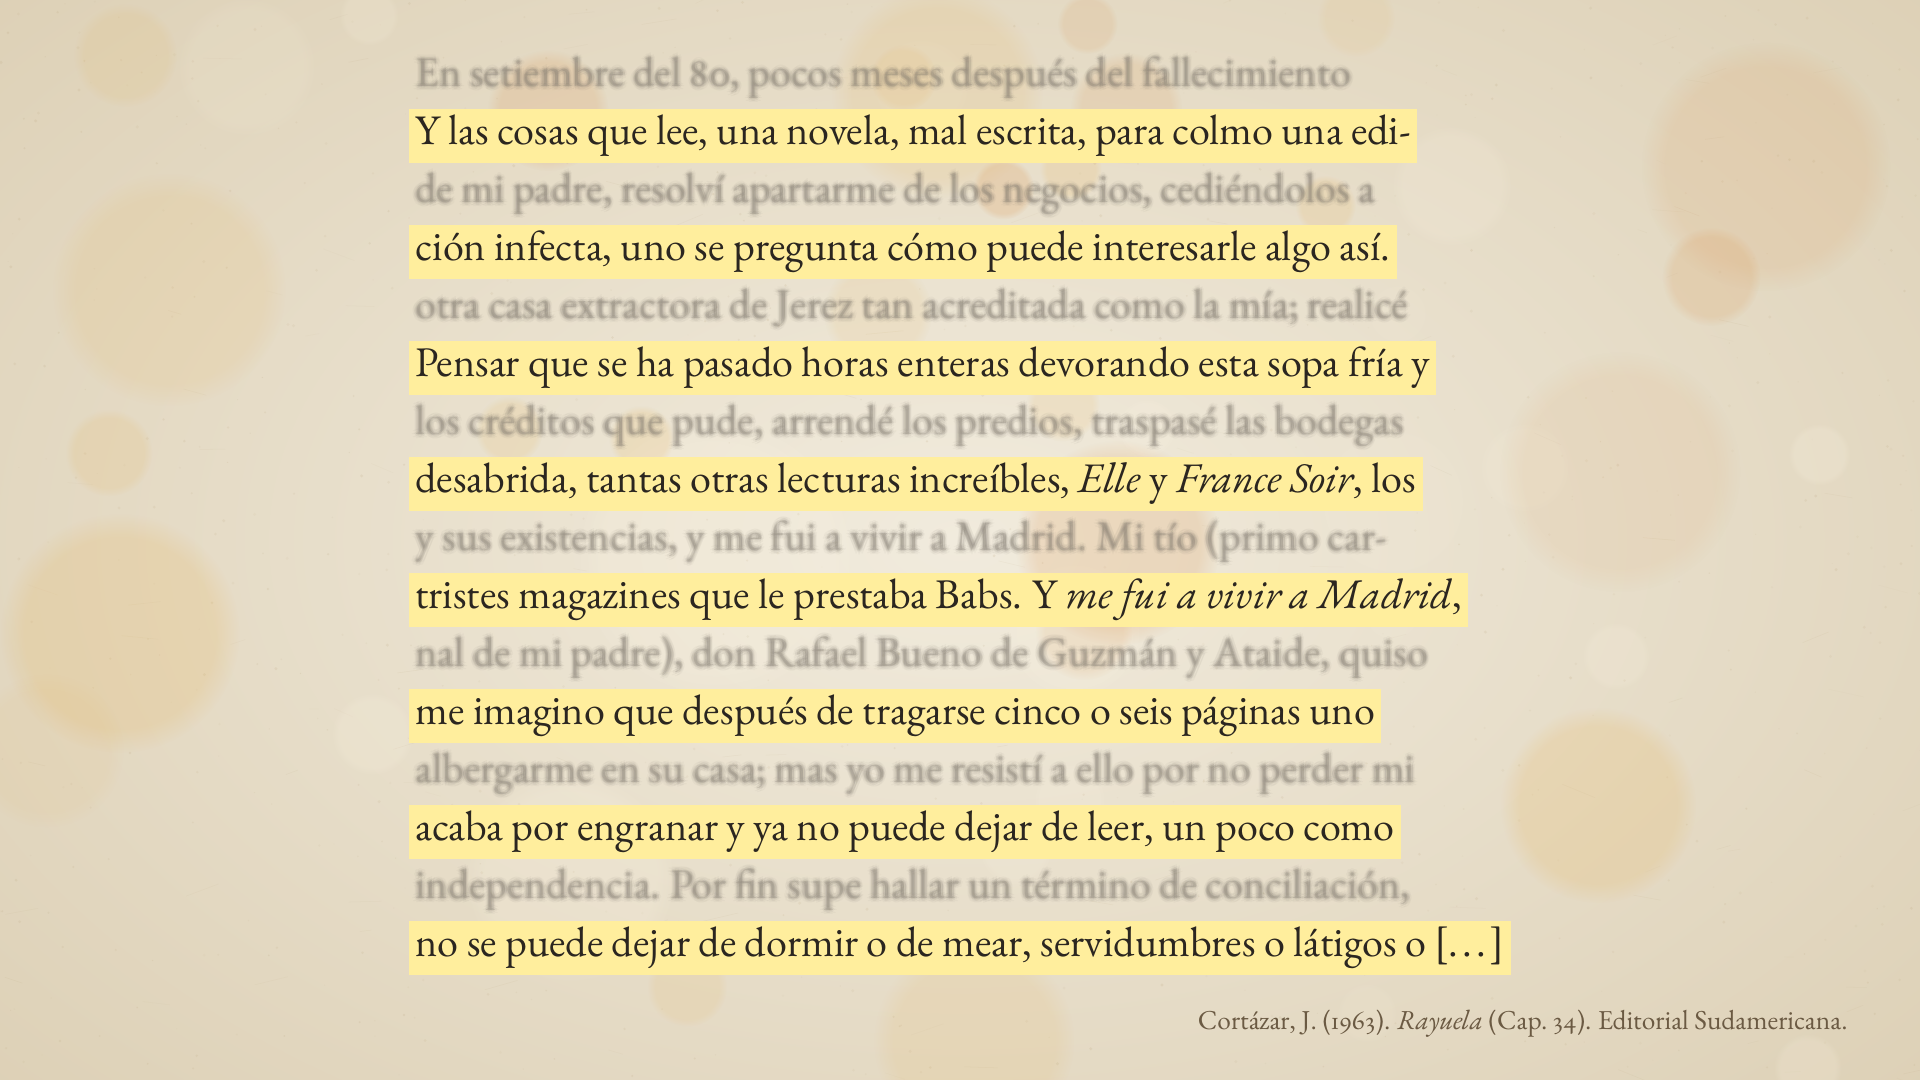
\includegraphics[width=0.85\textwidth]{Resources/img/Dinamica3/Fase2/Dinamica3_Fase2_Diapositiva2.png}
  \caption{Diapositiva 2 de la Fase 2: la novela difuminada y Oliveira en primer plano.}
  \label{fig:fase2d2}
  \fuentefigura{Elaboración propia. Texto: \citet[cap.~34, p.~212]{cortazar1963}.}
\end{figure}

\textbf{Diapositiva 3: el lenguaje digerido.} Fondo oscuro y limpio, con los dos hilos separados y resumidos en lenguaje cotidiano (figura~\ref{fig:fase2d3}). El resumen evidencia el resultado del procesamiento analítico.

\begin{figure}[H]
  \centering
  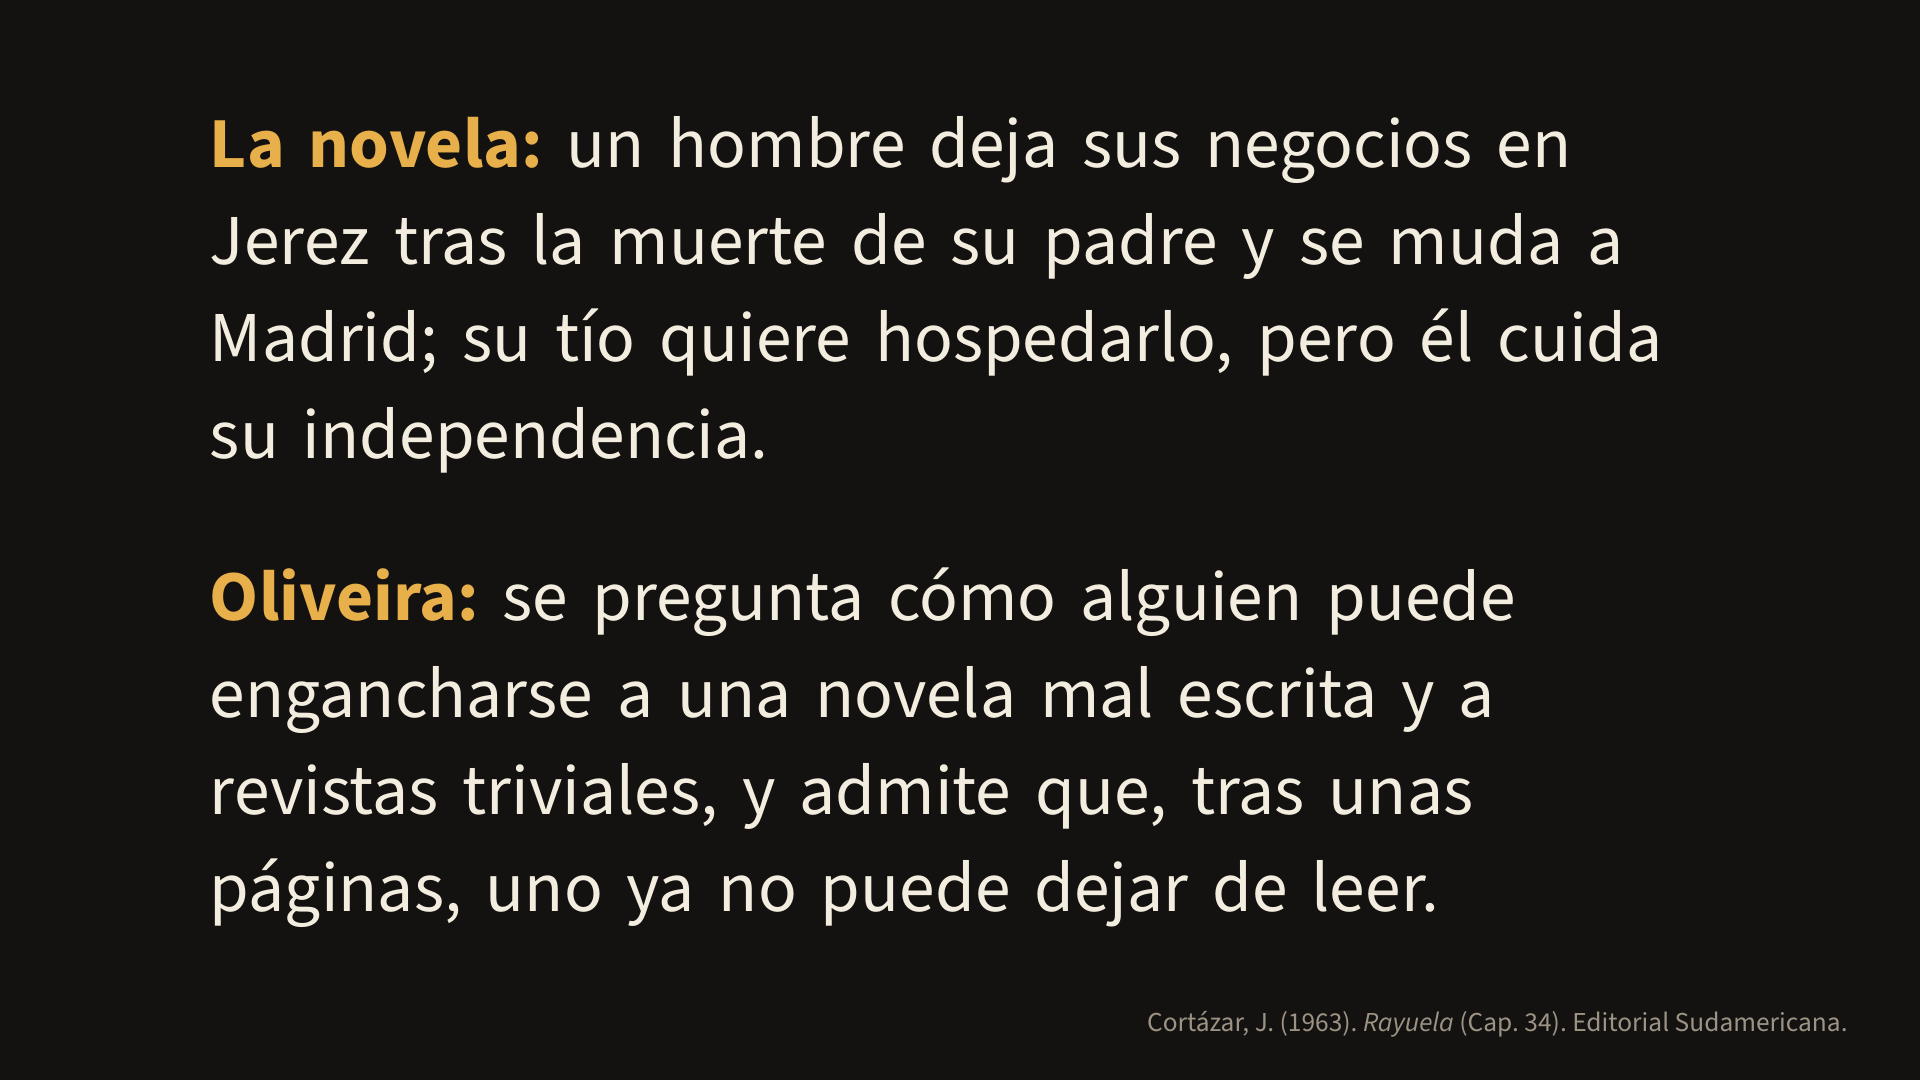
\includegraphics[width=0.85\textwidth]{Resources/img/Dinamica3/Fase2/Dinamica3_Fase2_Diapositiva3.png}
  \caption{Diapositiva 3 de la Fase 2: el resumen de los dos hilos.}
  \label{fig:fase2d3}
  \fuentefigura{Elaboración propia a partir de \citet[cap.~34]{cortazar1963}.}
\end{figure}

\subsubsection*{Fase 3: hiperfoco quebrándose (meltdown)}

Esta fase se proyecta con el audio en su punto alto. Su propósito es simular la sobrecarga sensorial que antecede a un meltdown y la pérdida de la capacidad de procesar el significado del lenguaje.
% EDITAR: confirmar intervalo del audio (propuesta: 10:34 – 13:57, tinnitus
%         agudo, antes de la meseta final).

\textbf{Diapositiva 1: lectura con tensión.} Se proyecta de nuevo el resumen de la Fase~2, un texto en español limpio que el grupo ya comprendió, mientras el audio comienza a volverse molesto. El pergamino se oscurece en los bordes y aparecen las primeras luces saturadas (figura~\ref{fig:fase3d1}).

\begin{figure}[H]
  \centering
  \includegraphics[width=0.85\textwidth]{Resources/img/Dinamica3/Fase3/Dinamica3_Fase3_Diapositiva1.png}
  \caption{Diapositiva 1 de la Fase 3: lectura con tensión.}
  \label{fig:fase3d1}
  \fuentefigura{Elaboración propia a partir de \citet[cap.~34]{cortazar1963}.}
\end{figure}

\textbf{Diapositiva 2: la falla del filtro.} El fondo se llena de luces bokeh agresivas, grandes y saturadas, y el texto se desenfoca severamente; ya no hay una capa nítida (figura~\ref{fig:fase3d2}). La lectura exige un esfuerzo visual alto bajo el ruido: incluso lo que ya se había comprendido se vuelve difícil de recuperar.

\begin{figure}[H]
  \centering
  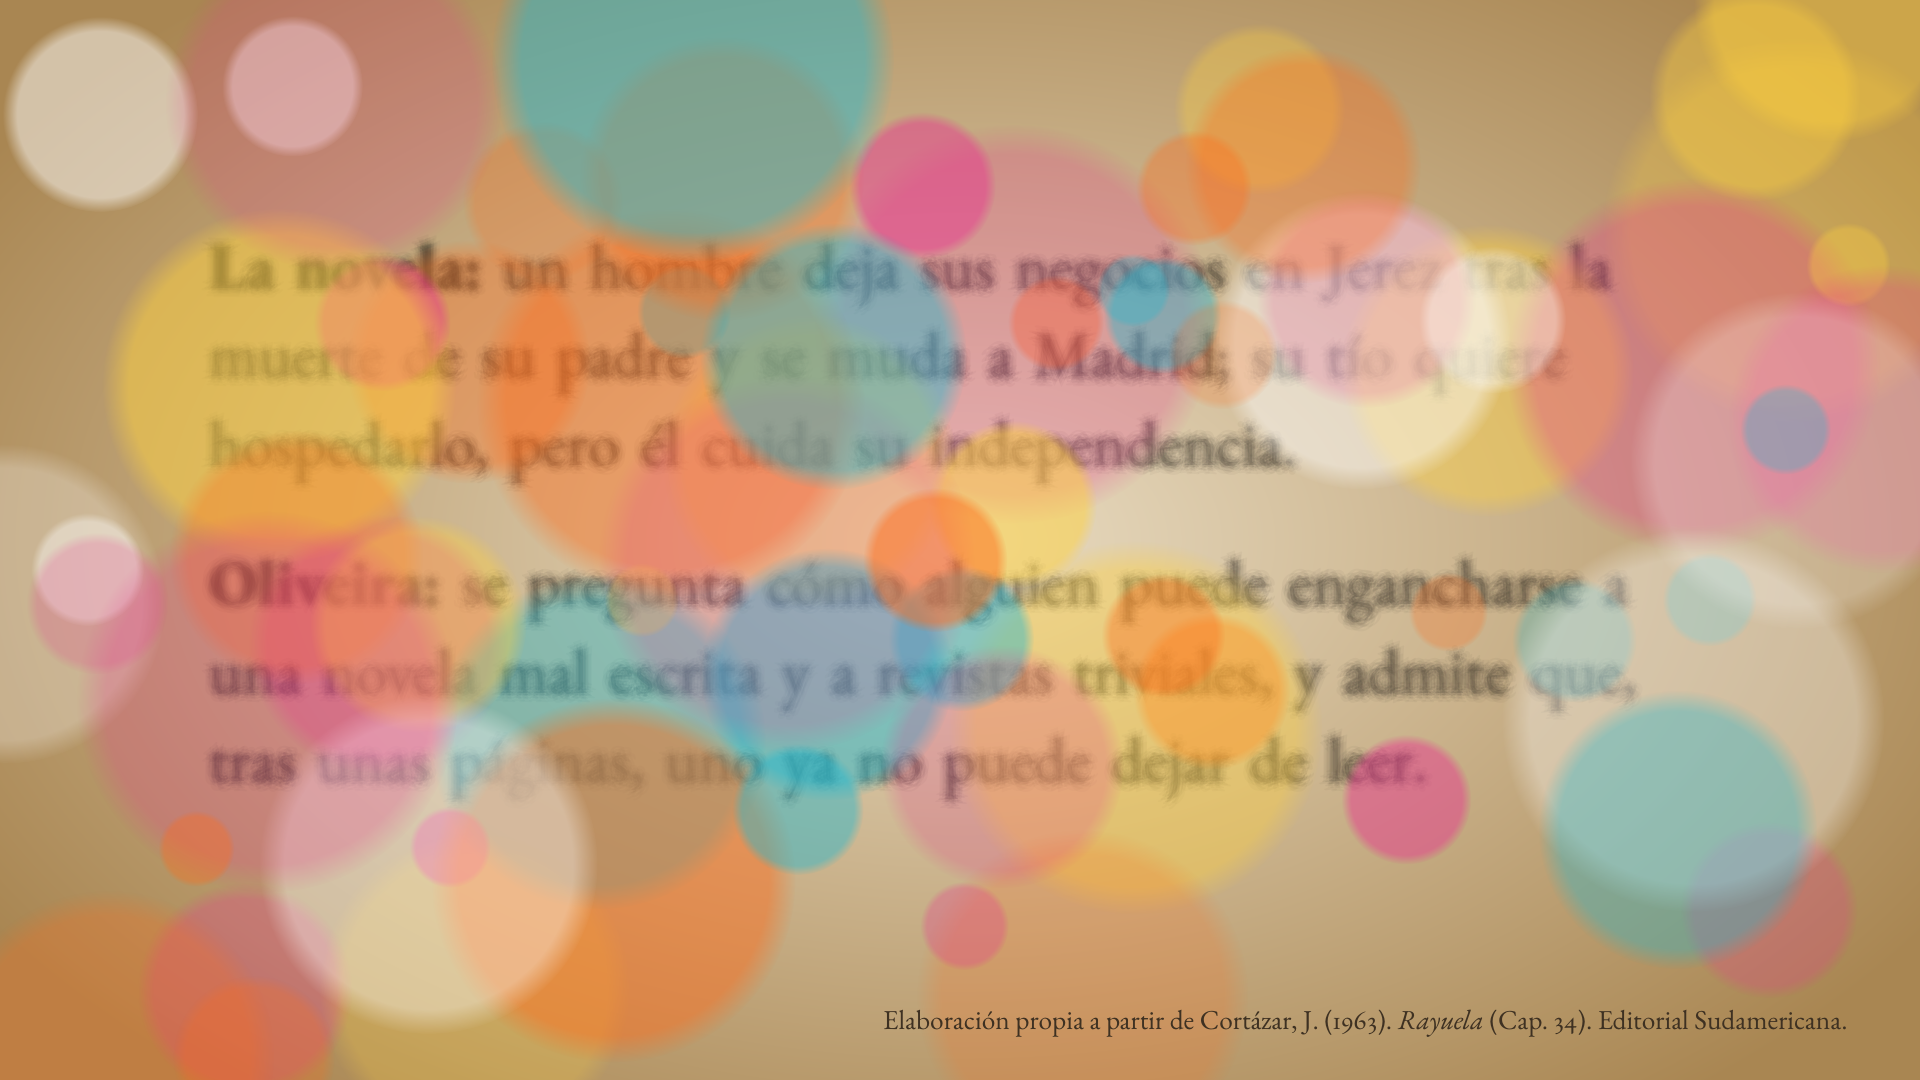
\includegraphics[width=0.85\textwidth]{Resources/img/Dinamica3/Fase3/Dinamica3_Fase3_Diapositiva2.png}
  \caption{Diapositiva 2 de la Fase 3: la falla del filtro.}
  \label{fig:fase3d2}
  \fuentefigura{Elaboración propia a partir de \citet[cap.~34]{cortazar1963}.}
\end{figure}

\textbf{Diapositiva 3: el quiebre al glíglico.} Se proyecta textualmente el inicio del capítulo 68, nítido y sobre el pergamino limpio de la Fase~1 (figura~\ref{fig:fase3d3}). Representa el punto en que, aunque las letras se ven con claridad, la mente ya no puede descifrar su significado.

\begin{figure}[H]
  \centering
  \includegraphics[width=0.85\textwidth]{Resources/img/Dinamica3/Fase3/Dinamica3_Fase3_Diapositiva3.png}
  \caption{Diapositiva 3 de la Fase 3: el inicio del capítulo 68.}
  \label{fig:fase3d3}
  \fuentefigura{Elaboración propia. Texto: \citet[cap.~68]{cortazar1963}.}
\end{figure}

\subsubsection*{Clímax y corte}

\begin{enumerate}
  \item \textbf{Escalada sensorial.} La intensidad del audio crece por acumulación de capas hasta representar el punto de sobrecarga que antecede a un meltdown. A la carga auditiva se suman colores saturados en la proyección y luces molestas en el aula.
  \item \textbf{Corte.} El audio se interrumpe de tajo y se sustituye por ruido blanco, y la pantalla queda en blanco. En ese momento se explica el shutdown.
\end{enumerate}
% EDITAR: momento en que se activan colores saturados y luces; tipo de iluminación.

\textbf{Vínculo con la teoría.} Los estímulos elegidos corresponden a los que reportan \citet{jones2020} en el aula, como luces brillantes, ruido y entornos \enquote{demasiado saturados visualmente}, y a los \enquote{estímulos sensoriales aversivos abrumadores} que \citet{phung2021} señalan entre los detonantes del meltdown. El corte final evoca la descripción del shutdown como una experiencia en la que la persona \enquote{se retira de su entorno} \citep{phung2021}.

% =============================================================================
%  5-Conclusiones.tex
% =============================================================================

\section{Conclusiones y reflexión final}

% EDITAR: barreras sensoriales y cognitivas; responsabilidad del urbanista y del docente.
\textit{[Sección pendiente de desarrollo.]}

\subsection{Experiencia personal}

% EDITAR: placeholder — se desarrollará en otra sesión.
\textit{[Sección pendiente de desarrollo.]}

% =============================================================================
%  6-Preguntas.tex
% =============================================================================

\section{Preguntas para la autorreflexión y la crítica}

% EDITAR: 4 a 5 preguntas abiertas sobre diseño de ciudades y aulas desde la neurotipicidad.
\textit{[Sección pendiente de desarrollo.]}


% ── Bibliografía ──────────────────────────────────────────────────────────────
\clearpage
\bibliographystyle{apalike}
\bibliography{referencias}

\end{document}
